\setcounter{table}{0}
\setcounter{figure}{0}
\renewcommand{\thefigure}{S\arabic{figure}}
\renewcommand{\thetable}{S\arabic{table}}

\appendix

\chapter{Evaluations to determine the final genotype calling model}\label{chiamantesup}
We have described our genotype calling method with a number of possible different variations on the model:
\begin{itemize}
  \item choice of distribution for array data - bivariate Gaussian or \st with $\upsilon=5$
  \item three possible prior distributions for the cluster centroids, $\mu$
  \item prior allele frequency distribution $\alpha$    
%  \item constant value for failure density $P(Y|Z^Y=1)$
\end{itemize}
We evaluated these options using chromosome 20 Omni2.5S data for 1,525 individuals (described in section~\ref{chap2:data}).  Concordance with the Affymetrix data (equation~\ref{concordance}) was evaluated for different parameterisations of the genotype calling method and was used (amongst other considerations) to determine the final choice of model that was used in our final comparisons with other genotype calling software in section~\ref{chap2:results:comparison}.  We assessed both the array-only scenario (1,525 individuals assayed on Illumina's chip) and the mixed array and sequence scenario (1094 of these individuals having 4X sequence data).

\section*{Choice of centroid priors and distribution} \label{centroidcompare}
\label{chap2:results:centroid}
When making genotype calls using only array data, the combination of the \st distribution and the third choice of priors (correlated centroids) performed the most accurately, albeit slightly, across the range of posterior probability thresholds (Figure~\ref{priorcompare}).  When the genotype calls were made with both array and sequence data, the \st distribution again performed better than the Gaussian, but the priors appear to have little effect on accuracy.  This makes intuitive sense as we have more data in this scenario, hence the priors are having limited effect on parameter estimates.  Given these results, we chose to use the mixture of \st distributions with the third choice of priors (Equation~\ref{model3}).

\begin{figure}[h]
  \begin{center} 
    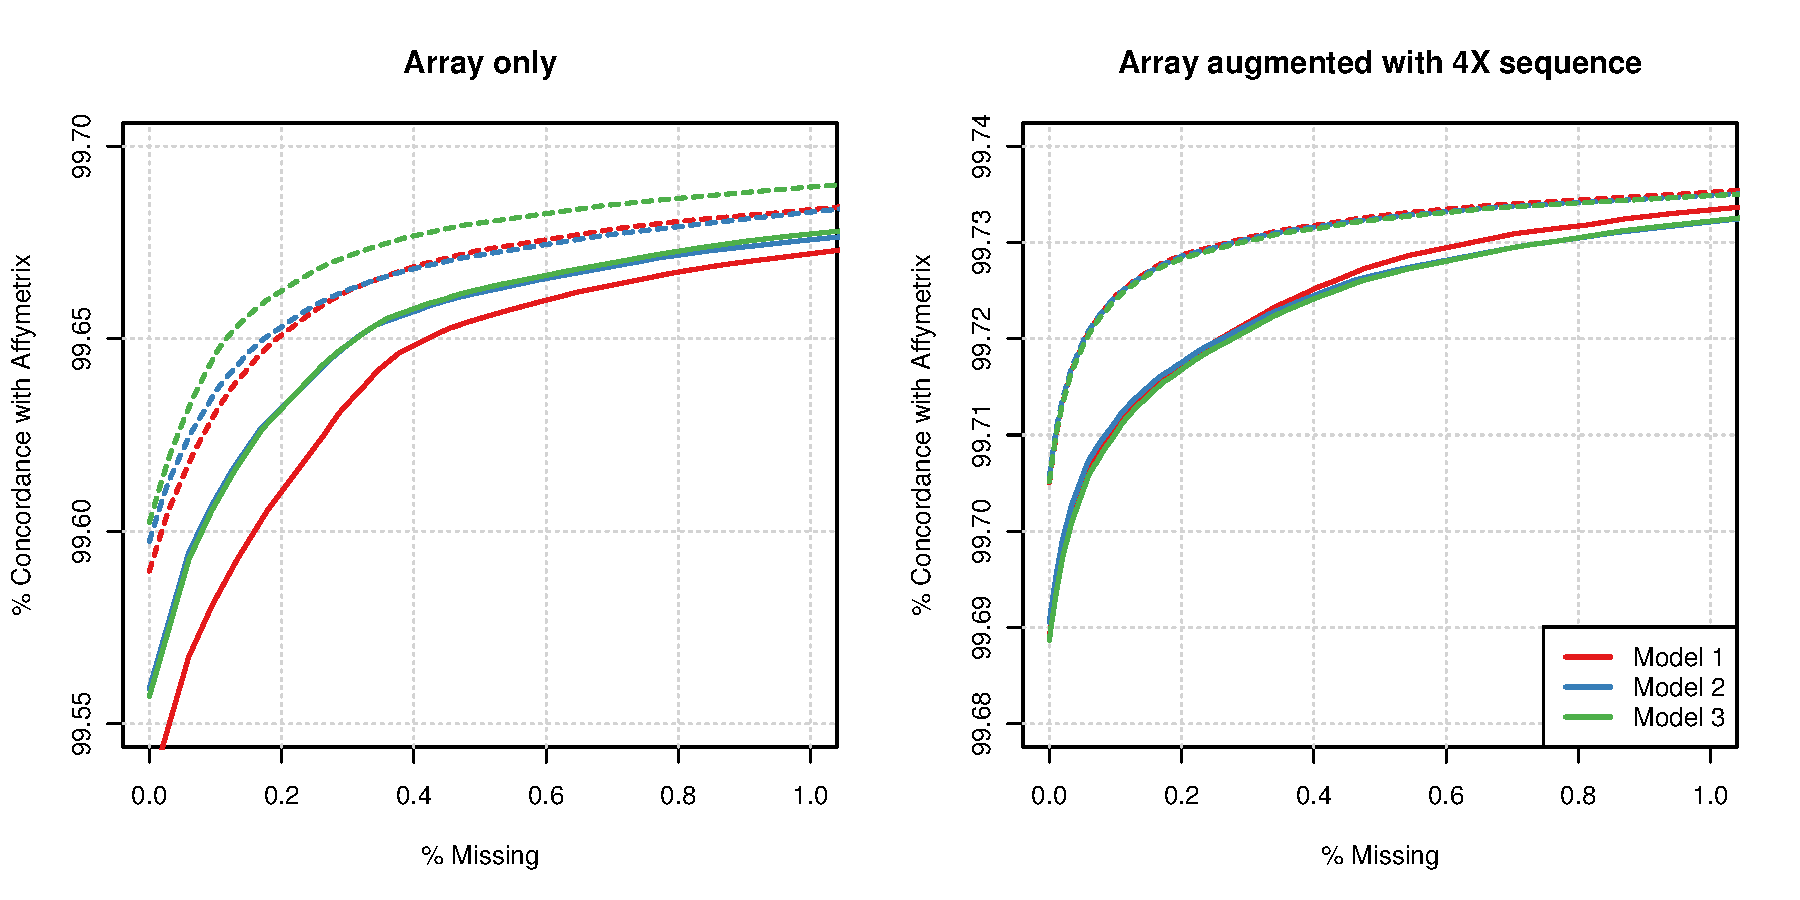
\includegraphics[width=\textwidth]{chap2figs/SupFig4}
    \caption[Evaluation of prior choices for centroids]{Comparison of our three possible choices of priors (coloured) and a mixture of Gaussian distributions (solid lines) versus a mixture of \st distributions with $\upsilon=5$ (dashed lines) for array only calls (left) and array data augmented with sequence data (right).  We can see that \st is consistently more accurate for both data sets and all choices of priors.  In the array only context, our third prior performs the most accurately (albeit slightly) when combined with the \st distribution.  Whilst when sequence data is included in the modelling, the choice of prior appears to have limited effect on accuracy.  Note the vertical scale varies between the plots, that is, the array augmented with sequence calls are $\approx$ 0.1\% more accurate than the array-only calls.\label{priorcompare}}
  \end{center} 
\end{figure}


\subsection*{Choice of allele and genotype frequency prior} \label{freqprior}
\label{chap2:results:exploratory:freq}
In section~\ref{chap2:priors} we described a flat Beta prior for the reference allele frequency. A well known result in population genetics~\citep{fu1995statistical} states that the distribution of alternate allele frequencies ($\alpha$ in our model) is inversely proportional to the frequency, that is $P(\alpha) \propto 1/\alpha$.  This result is not necessarily consistent with the loci frequencies present on a microarray.  We took an empirical approach to modelling the allele frequency spectrum of loci on the Omni2.5S chip. Loci information was downloaded from the 1000 Genomes FTP server \footnote{\url{ftp://ftp.1000genomes.ebi.ac.uk/vol1/ftp/release/20110521/ALL.wgs.phase1_release_v3.20101123.snps_indels_sv.sites.vcf.gz}}, global allele frequencies for the Omni 2.5S positions were then extracted from this file and we estimated parameters for the Beta(a,b) distribution using maximum likelihood ($\hat{a}=0.363,\hat{b}=1.254$).  The fit of this distribution appears very reasonable (Figure~\ref{AFS_betafit}).


\begin{figure}[h]
\begin{center} 
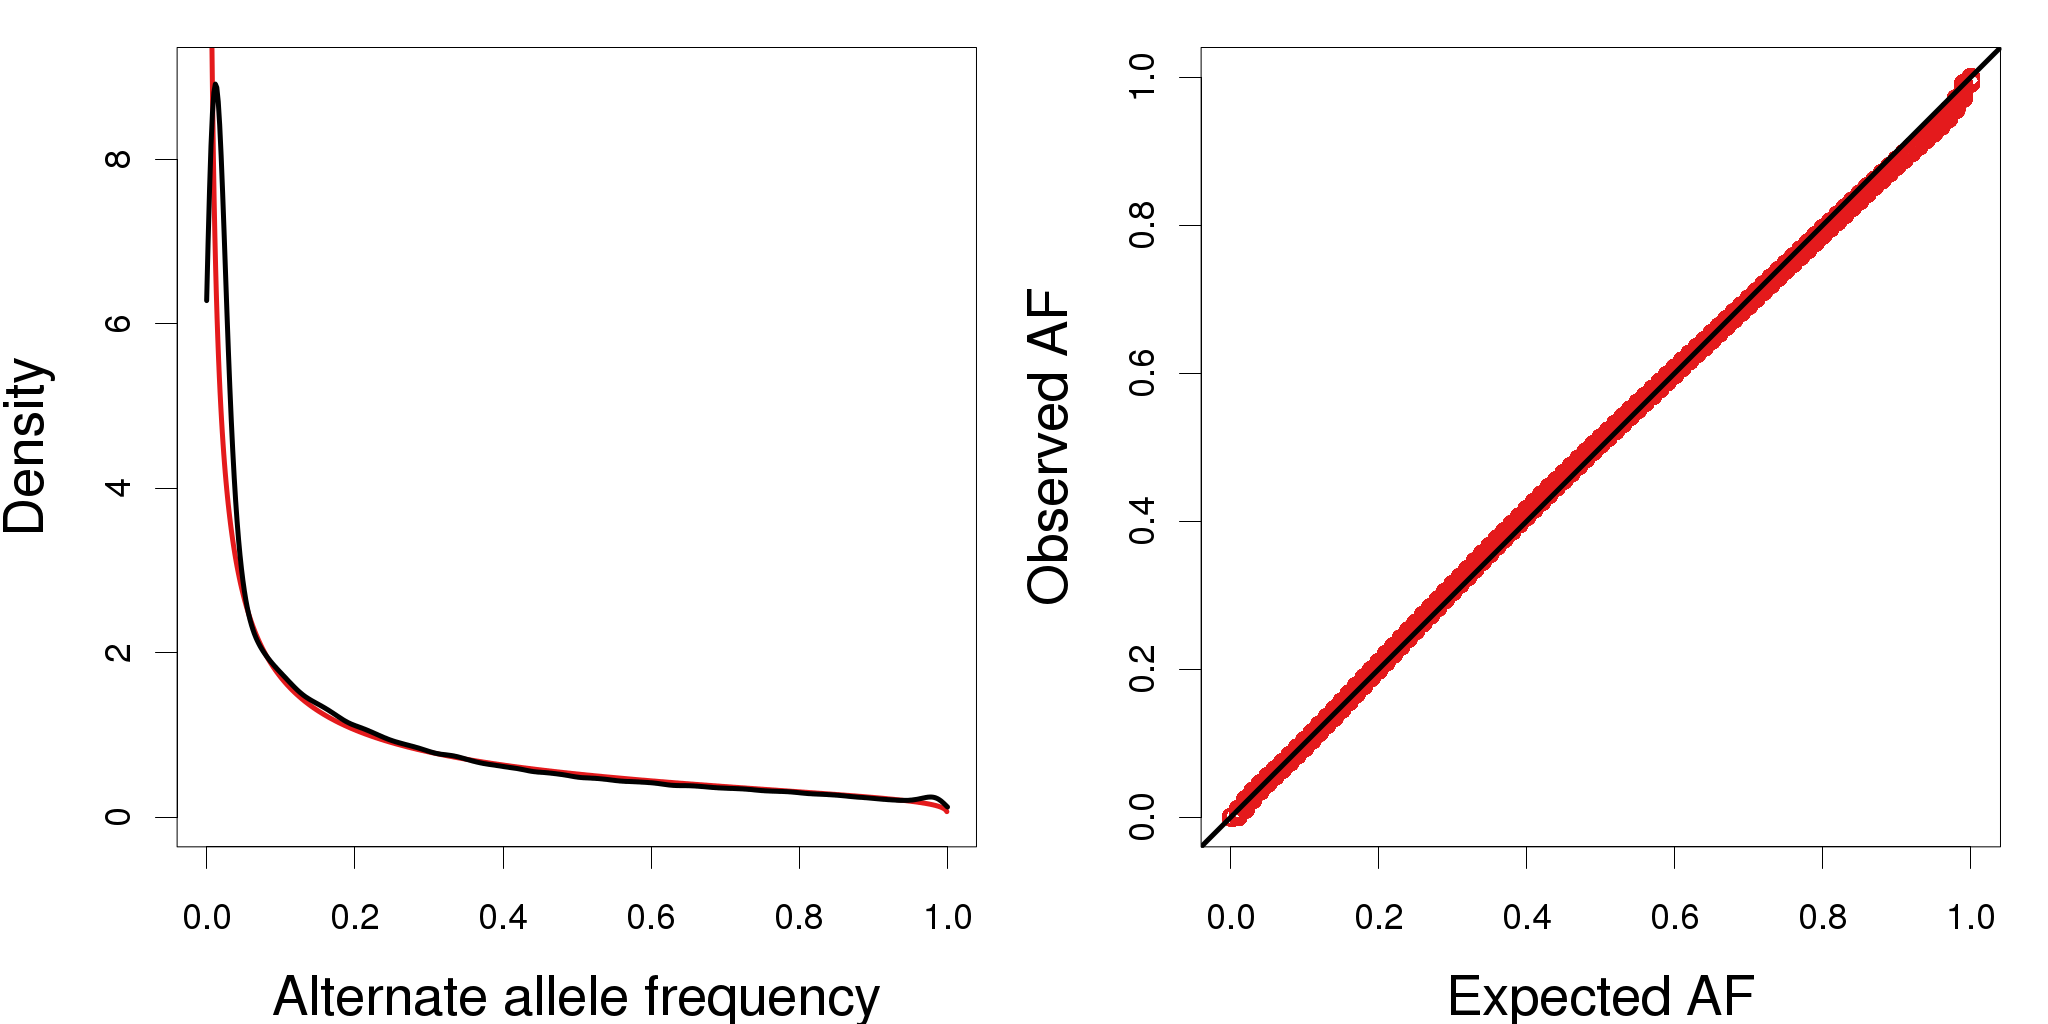
\includegraphics[width=\textwidth]{chap2figs/SupFig2}
\caption[Allele frequency spectrum on Omni2.5S chip]{\textbf{Left:} Kernel smoothed density estimate of the alternate allele frequency spectrum on the Omni2.5S chip (black) and a Beta distribution fitted to these frequencies.  \textbf{Right:} Q-Q plot of the empirical quantiles of the frequencies against theoretical quantiles of the Beta distribution.
\label{AFS_betafit}}
\end{center} 
\end{figure}
\clearpage
We used a Dirichlet prior for the genotype frequencies that allows some deviation from Hardy-Weinberg Equilibrium. After one generation of random breeding a population will be in HWE.  However, in a case-control GWAS the cases may deviate from HWE due to biased sampling of causative alleles so allowing some departure from HWE may be desirable.

To investigate the effect of our choice of priors on accuracy we called genotypes using only array data on the 1,525 samples for all loci on chromosome 20 using five different priors. 

\begin{enumerate}\label{freqpriorlist}
\item a flat Beta prior for reference allele frequency with departure from HWE allowed ($\delta=10$)
\item a flat Beta prior for reference allele frequency with \emph{no departure} from HWE allowed
\item the estimated Beta distribution for reference allele frequencies with departure from HWE allowed ($\delta=10$)
\item the estimated Beta distribution for reference allele  \emph{no departure} from HWE allowed
\item a flat Dirichlet prior for genotype frequencies $\lambda \sim \textrm{Dirichlet}(1,1,1)$
\end{enumerate}

We found the forced HWE priors to be slightly more accurate than our Dirichlet prior (with some HWE penalty) and than the flat Dirichlet prior with no HWE deviation penalty (Figure~\ref{freq_prior_comparison}).  However, in case-control GWAS allowing deviation from HWE may be desirable.  Whilst the Beta prior estimated from population data was (marginally) more accurate we left the Beta prior as flat since this accuracy is conceivably due to over fitting.  In any case, the choice of priors for $\alpha$ and $\lambda$ clearly have a limited effect on accuracy. We leave $\delta$ as a tuneable parameter in our software (with $\delta=10$ as the default value). 

\begin{SCfigure}[1][h]
\centering
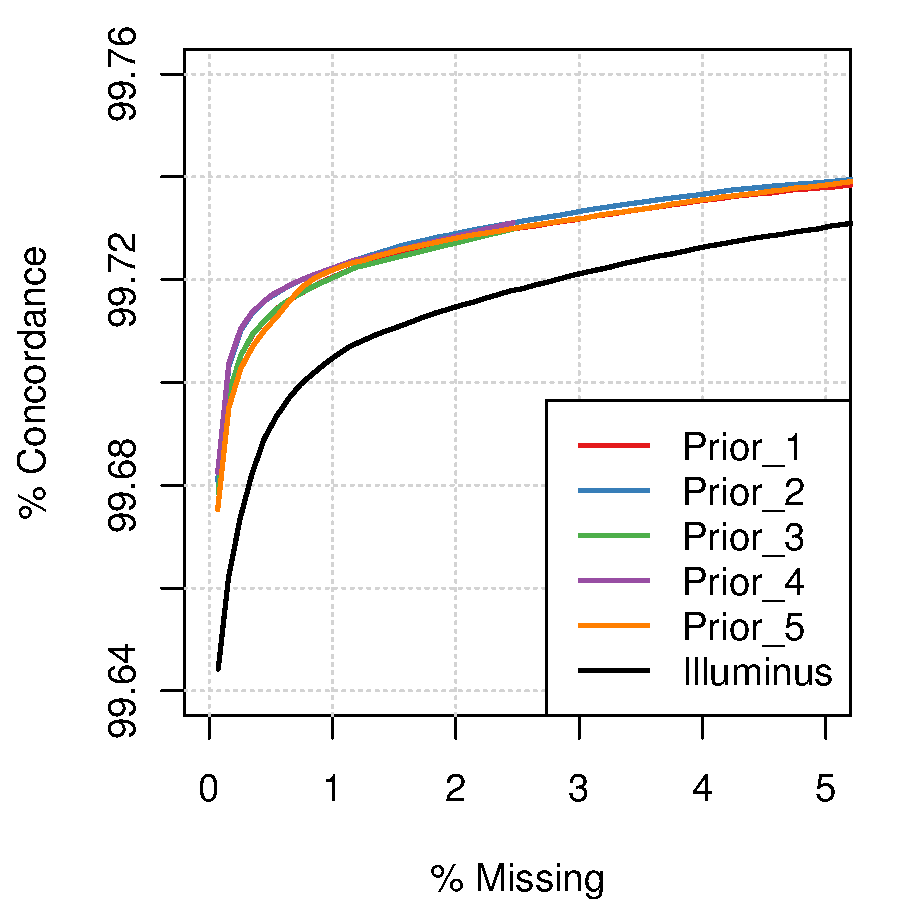
\includegraphics[width=.5\textwidth]{chap2figs/SupFig3}
\caption[Evaluation of prior choices for allele frequency]{Concordance against missing data rate for five different priors described in~\ref{freqpriorlist}; \textbf{1.} a flat Beta prior for reference allele frequency with departure from HWE allowed ($\delta=10$ in Eq. 2)
\textbf{2.} a flat Beta prior for reference allele frequency with \emph{no departure} from HWE allowed
\textbf{3.} the estimated Beta distribution for reference allele frequencies with departure from HWE allowed ($\delta=10$ in Eq. 2)
\textbf{4.} the estimated Beta distribution for reference allele  \emph{no departure} from HWE allowed
\textbf{5.} a flat Dirichlet prior for genotype frequencies $\lambda \sim \textrm{Dirichlet}(1,1,1)$
\label{freq_prior_comparison}}
\end{SCfigure}


%% \subsubsection{Choice of sequence failure density} 
%% \label{chap2:results:fail_dens}
%% There was no obvious way to choose a value for $P(Y_i|Z_{Y_i}=1)=h_Y(y_i)$ and a constant value is likely to be overly simplistic.  Realistically it should be some function of typical sequencing QC measures such as coverage, mapping quality and base quality. However this was beyond the scope of our method which aims to leverage sequence data in a simple manner to improve the accuracy of genotype microarry data. Hence we undertook a simple empirical experiment, trying a range of values for $h_Y(y_i)$ and calculating concordance (Figure~\ref{fail_dens}). We found that actually setting $h_Y(y_i)=0.01$ leads to extremely marginally better results than $h_Y(y_i)=0.0$ and as $h_Y(y_i)$ increases the accuracy tends to what we see when no sequencing data is used (not surprisingly).  This result may lead us to consider removing the failure indicator for sequencing data altogether but this is specious reasoning.  Due to false variant calls in the Pilot sequencin of the 1000 Genomes Project, roughly 8\% of sites on the Omni2.5S chip are monomorphic (supplementary table~\ref{chap2:locisummary} improvements in sequencing technology and bioinformatics also mean these sites are correctly called as monomorphic in sequencing data although some errors remain.  Loci that are present on both the Affymetic and Omni chips are more likely to be genuine SNPs and well ascertained by sequencing pipelines.  When we look at the the Q-Q plots (for \emph{all} Omni SNPs) for divergence from Hardy-Weinberg Equilibrium Figure~\ref{fail_dens} (right) for differing values of $h_Y(y_i)$ we can see for $h_Y(y_i)=0$

%% .Section~\ref{chap2:results:errors} also shows some futher utility of the sequence failure indicator variable.

%% \begin{figure}[ht!]
%% \begin{center} 
%%   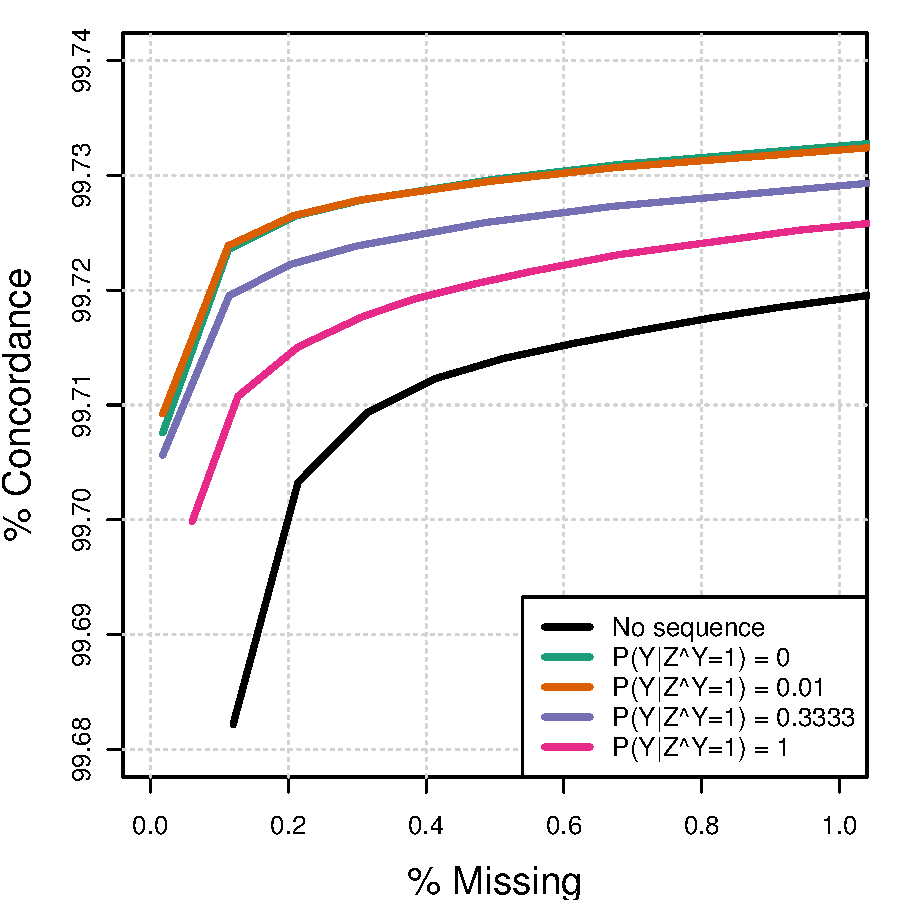
\includegraphics[width=.5\textwidth]{chap2figs/SupFig12}
%% \caption{Concordance with Axiom against missing data rate for varying values of $P(Y|Z^Y=1)$ on chromsome 20.  Calls were made using 1525 inviduals assayed on the Omni2.5S data, a subset of 1094 individuals were also sequenced at 4X.  Calls from Chiamante using only array data are included for scale. \label{fail_dens}}
%% \end{center} 
%% \end{figure}


\chapter{Supplemental Tables}
\begin{table}[ht]\footnotesize
\begin{center}
\begin{tabular}{ |r|rrrrrr|}
\hline
& Illumina  & Affymetrix & 4X &  Omni2.5S & Omni2.5S & Omni2.5S/\\
Population &  Omni2.5S & Axiom & sequence & 4Xsequence & Axiom &Axiom/ \\
& & & & &&Sequence \\
\hline

ASW & 96 & 90 & 61 & 61 & 88 & 53 \\ 
CEU & 104 & 180 & 87 & 87 & 101 & 84 \\ 
CHB & 100 & 90 & 97 & 97 & 86 & 85 \\ 
CHD & 0 & 90 & 0 & 0 & 0 & 0 \\ 
CHS & 150 & 0 & 100 & 100 & 0 & 0 \\ 
CLM & 107 & 0 & 60 & 60 & 0 & 0 \\ 
FIN & 100 & 0 & 93 & 93 & 0 & 0 \\ 
GBR & 96 & 0 & 89 & 89 & 0 & 0 \\ 
GIH & 0 & 90 & 0 & 0 & 0 & 0 \\ 
IBS & 69 & 0 & 14 & 14 & 0 & 0 \\ 
JPT & 100 & 91 & 89 & 89 & 91 & 80 \\ 
LWK & 100 & 90 & 97 & 97 & 90 & 87 \\ 
MKK & 31 & 180 & 0 & 0 & 31 & 0 \\ 
MXL & 100 & 90 & 66 & 66 & 90 & 56 \\ 
PUR & 111 & 0 & 55 & 55 & 0 & 0 \\ 
TSI & 100 & 90 & 98 & 98 & 90 & 90 \\ 
YRI & 161 & 180 & 88 & 88 & 161 & 88 \\ 
\hline
ALL & 1525 & 1261 & 1094 & 1094 & 828 & 623 \\ 
\hline

\end{tabular}
\caption[Summary of 1000 Genomes data used in genotype calling]{Summary of the samples that have been assayed on the three technologies as well as the intersections of these technologies.\label{sampleinfo}}
\label{chap2:sampleinfo}
\end{center}
\end{table}

\begin{table}
\begin{center}
\begin{tabular}{|l|r|rr|rr|rr|}
\hline
\multicolumn{8}{|c|}{Chiamante (no sequence)}\\
\hline
&&\multicolumn{2}{c}{828}&\multicolumn{2}{|c}{623}&\multicolumn{2}{|c|}{205}\\
\hline
Filter & SCR & GCR & Conc & GCR & Conc & GCR & Conc \\ 
\hline
None & 100.000 & 99.824 & 99.696 & 99.838 & 99.695 & 99.788 & 99.696 \\ 
GCR & 99.765 & 99.646 & 99.698 & 99.661 & 99.698 & 99.607 & 99.698 \\ 
HWE & 99.941 & 99.766 & 99.708 & 99.781 & 99.708 & 99.730 & 99.707 \\ 
PP & 100.000 & 99.744 & 99.715 & 99.767 & 99.714 & 99.686 & 99.717 \\ 
\hline
GCR+HWE & 99.710 & 99.590 & 99.709 & 99.605 & 99.710 & 99.552 & 99.709 \\ 
PP+GCR & 99.694 & 99.520 & 99.722 & 99.545 & 99.722 & 99.457 & 99.724 \\ 
PP+HWE & 99.940 & 99.696 & 99.722 & 99.719 & 99.722 & 99.636 & 99.724 \\ 
\hline
All & 99.659 & 99.486 & 99.726 & 99.511 & 99.726 & 99.423 & 99.728 \\ 
\hline
\end{tabular}
% \caption{SCR, GCR and concordance with Axiom data for a call set produced using Chiamante with Omni2.5S data on 1525 1000 Genomes individuals (no sequence data was used in this analysis). 
% Metrics were calculated on 828 inviduals with Axiom data available, and then on the same 828 individuals split into two groups; 623 who had 4X sequence data available and 205 who had no sequence data available.
% }
% \end{center}
% \end{table}

% \begin{table}[ht]
% \begin{center}
~\\
~\\
\begin{tabular}{|l|r|rr|rr|rr|}
\hline
\multicolumn{8}{|c|}{Chiamante + Sequence}\\
\hline
&&\multicolumn{2}{c}{828}&\multicolumn{2}{|c}{623}&\multicolumn{2}{|c|}{205}\\
\hline
Filter & SCR & GCR & Conc & GCR & Conc & GCR & Conc \\ 
\hline
None & 100.000 & 99.986 & 99.721 & 100.000 & 99.723 & 99.950 & 99.714 \\ 
GCR & 99.985 & 99.974 & 99.722 & 99.985 & 99.724 & 99.946 & 99.715 \\ 
HWE & 99.984 & 99.970 & 99.723 & 99.984 & 99.725 & 99.934 & 99.716 \\ 
PP & 100.000 & 99.940 & 99.733 & 99.968 & 99.734 & 99.869 & 99.729 \\ 
\hline
GCR+HWE & 99.969 & 99.958 & 99.723 & 99.969 & 99.726 & 99.930 & 99.717 \\ 
PP+GCR & 99.966 & 99.914 & 99.734 & 99.938 & 99.736 & 99.853 & 99.731 \\ 
PP+HWE & 99.986 & 99.927 & 99.734 & 99.955 & 99.735 & 99.856 & 99.730 \\ 
\hline
All & 99.954 & 99.903 & 99.736 & 99.927 & 99.737 & 99.841 & 99.732 \\ 
\hline
\end{tabular}
\caption[Breakdown of genotype calling performing for
sequenced/non-sequenced samples]{\textbf{Top:} SCR, GCR and concordance with Axiom data for a call set produced using Chiamante with Omni2.5S data on 1525 1000 Genomes individuals (no sequence data was used in this analysis).  Metrics were calculated on 828 individuals with Axiom data available, and then on the same 828 individuals split into two groups; 623 who had 4X sequence data available and 205 who had no sequence data available. \textbf{Bottom:} The same metrics for a call set produced with the same array data, but augmented with sequence information from a subset of 1094 individuals. We can see that there is an improvement in call rate and accuracy not only for the 623 individuals with sequence data, but also for the 205 individuals without sequence data.\label{chap2:results:splitchi}}
\end{center}
\end{table}


%% \begin{table}[ht]
%% \begin{center}
%% \begin{tabular}{rrrrrr}
%%   \hline
%%  Chromosome & Omni2.5S & BCM GLs & Axiom & Omni\_Axiom & All \\ 
%%   \hline
%%    1 & 191197 & 174203 & 441079 & 95930 & 95381 \\ 
%%  2 & 200037 & 183761 & 517849 & 108980 & 108392 \\ 
%%  3 & 167887 & 154328 & 459423 & 95341 & 94843 \\ 
%%  4 & 157357 & 144584 & 456698 & 89225 & 88700 \\ 
%%  5 & 149731 & 137635 & 412448 & 83865 & 83356 \\ 
%%  6 & 150265 & 137805 & 399701 & 84366 & 83846 \\ 
%%  7 & 133887 & 122945 & 335660 & 70574 & 70204 \\ 
%%  8 & 129541 & 119866 & 358241 & 72427 & 72042 \\ 
%%  9 & 107141 & 99329 & 258727 & 56843 & 56544 \\ 
%%  10 & 123548 & 113569 & 287587 & 63239 & 62880 \\ 
%%  11 & 120676 & 110840 & 281381 & 61709 & 61354 \\ 
%%  12 & 116228 & 106306 & 278340 & 61740 & 61364 \\ 
%%  13 & 85737 & 78986 & 232032 & 48592 & 48297 \\ 
%%  14 & 79307 & 73150 & 192567 & 42439 & 42214 \\ 
%%  15 & 74520 & 68661 & 166476 & 38813 & 38591 \\ 
%%  16 & 80838 & 74748 & 153351 & 35699 & 35526 \\ 
%%  17 & 70478 & 64676 & 111189 & 26903 & 26780 \\ 
%%  18 & 70476 & 65391 & 186324 & 39786 & 39550 \\ 
%%  19 & 52612 & 48034 & 56590 & 15256 & 15177 \\ 
%%  20 & 59114 & 55034 & 119865 & 28131 & 28029 \\ 
%%  21 & 33403 & 30738 & 79193 & 16809 & 16692 \\ 
%%  22 & 36064 & 33449 & 42188 & 11640 & 11504 \\ 
%% \hline
%%   All & 2390044 & 2198038 & 5826909 & 1248307 & 1241266 \\ 
%%    \hline
%% \end{tabular}
%% \caption{Number of autosomal SNPs present on the Omni2.5S chip, intersecting with BCM sequence likelihoods, Axiom and the intersection of all three pieces of data. Around 192006 ($\approx$ 8\%) of the chip positions were missing from the 1000G sequence genotype likelihoods but of these missing locations, only 7041 ($ \approx$ 0.3\%) were on the Axiom chip.}
%% \label{chap2:locisummary}
%% \end{center}
%% \end{table}

\chapter{Data sets}


\section*{Isolates data}
INGI-FVG and INGI-CARL: We would like to thank the people of the Friuli Venezia Giulia Region and of Carlantino for the everlasting support.

ORCADES: DNA extractions were performed at the Wellcome Trust Clinical Research Facility in Edinburgh. We would like to acknowledge the invaluable contributions of Lorraine Anderson and the research nurses in Orkney, the administrative team in Edinburgh and the people of Orkney.

Val Borbera: We thank the inhabitants of the Val Borbera for participating in the study, and the local administrations and the ASL-Novi Ligure for support, Fiammetta Vigan\`{o} for technical support and Professor Clara Camaschella for help with clinical data collection. 

CROATIA-Split, CROATIA-Vis, CROATIA-Korcula: We thank the inhabitants of the Split, Vis and Korcula for participating in the study.


\section*{WTCCC data}
This work makes use of data generated by the Wellcome Trust Case Control Consortium. A full list of the investigators who contributed to the generation of the data is available at \url{www.wtccc.org.uk}. Funding for the project was provided by the Wellcome Trust under awards 076113 and 085475.
